\chapter{Turbostratic carbons I: from cigarette butts}
\label{ch:cbs}

\newpage
\section*{Abstract}

Sequential \gls{htc} and KOH-mediated activation of \acrfullpl{ucf} has previously been shown by the author to provide a solution to the problem of \acrfull{cb} waste, in the form of an extremely promising \ce{H2} storage medium (see \ref{pub:CB}). The following study serves to expand the previous work \textit{via} carbonisation of \gls{hydrochar} derived from whole \acrfullpl{ucb} i.e. including the wrapping paper. \ce{KOH} activation of \acrshort{ucb}-\gls{hydrochar} yields carbons with much lower porosity than in \ref{pub:CB}, achieving micro-mesoporous carbons with $A_{BET}$ of up to \qty{1875}{\metre\squared\per\gram} and pore volume of \qty{0.89}{\cm\cubed\per\gram} at an activation temperature of \qty{700}{\degreeCelsius}. Thus, these materials are best applied to room temperature \ce{CO2} capture, with reasonable uptakes of \num{2.7} and \qty{14.1}{\milli\mole\per\gram} achieved at 1 and \qty{20}{\bar}, respectively.

\acrshortpl{ucb} are an unusual carbon precursor in that they contain a relatively high quantity, and diverse range of metals. As a result the composition and elemental distribution in \acrshortpl{ucb}, as well as in derived \glspl{hydrochar} and \glspl{turbostratic carbon} is investigated, as well as the efficacy of post-synthetic washing steps. \acrshortpl{ucb} and derived, unwashed \gls{hydrochar} were found to contain \ce{Al}, \ce{Fe}, \ce{K}, \ce{Mg}, \ce{Na}, \ce{Ti}, and \ce{Ca} in concentrations above \qty{0.10}{\mg\per\gram}. Many of these elements were also identified in derived \glspl{turbostratic carbon}. While it was hypothesised in \ref{pub:CB} that such contaminants may have an activating effect, there is no evidence of this in this work. Indeed, the stubbornness of these elements to removal \textit{via} \ce{HCl} washing results in porosity that is lower than expected indicating that these contaminants are limiting pore accessibility.

\newpage
\section{Introduction}

\acrfullpl{ucb} pose a large environmental hazard as a result of (i) being made of non-biodegradable \acrfull{ca} as well as (ii) containing a myriad of toxic chemicals.\citep{Slaughter2011, Puls2011, chevalier2018nano} As they are the most common waste material worldwide, there have been attempts to reduce their environmental presence, initially \textit{via} anti-littering campaigns.\citep{Prevention2011, Harris2011} More promising however is the prospect of valorising \acrshortpl{ucb} by various means, including conversion to activated carbons as reported by the author in \ref{pub:CB} as well as many other researchers.\citep{Soltani, Soltani2013, lima2018, xiong2019nitrogen, Lee2014, Hamzah2017, Yu2018, Wang2016a, Koochaki2019, Bilge2019}

\begin{figure}[h]
    \centering
    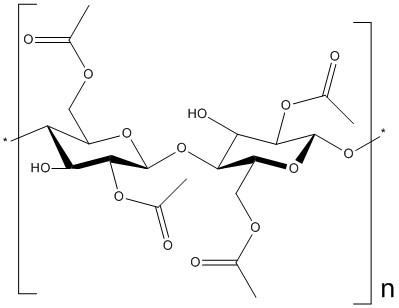
\includegraphics[width=0.7\columnwidth, keepaspectratio]{4-cbs/figs/cellulose_acetate.jpg}
    \caption{Structure of cellulose acetate.}
    \label{fig:cellulose acetate}
\end{figure}

\begin{sloppypar}
The reported porosity of carbons derived from \acrshortpl{ucb} is highly varied depending on synthetic conditions. In the absence of an \gls{activating agent}, and without pre-carbonisation steps, $A_{BET}$ typically does not exceed \qty{700}{\metre\squared\per\gram}.\citep{Koochaki2019, Soltani2013, Yazdi2012, Lee2014, Hamzah2017} Whereas using a \gls{porogen}, and/or pre-carbonising in air or hydothermally can improve surface areas to around \qty{3000}{\metre\squared\per\gram}.\citep{Xiong2018a, Koochaki2019, Sun2017, Bilge2019} The author's reports of ultrahigh porosity from KOH-activated hydrothermally carbonised \acrshortpl{ucb} in \ref{pub:CB} ($A_{BET}$ \qty{>4000}{\metre\squared\per\gram}, pore volume \qty{>2.00}{\cm\cubed\per\gram}) and high degree of microporosity (\qty{>90}{\percent}) are partially corroborated by the similar results using pure \acrfull{ca} in \ref{pub:CA}, suggesting that \acrshort{ca} is an ideal precursor for activation to yield high surface area carbons. Xiong \textit{et al.} also report a nitrogen-doped \acrshort{ucb}-derived activated carbon with hierarchical porosity and $A_{BET}$ of \qty{3420}{\metre\squared\per\gram}, though this result is dubious as (i) the \ce{N2} isotherm does not include ultralow pressure data, (ii) freespace appears to be incorrectly measured and (iii) isotherm measurement is not described in the text.\citep{xiong2019nitrogen} It was suggested in \ref{pub:CB} that the unusually high porosity of \acrshort{ucb}-derived carbons may be contributed to by the action of so-called contaminant-\glspl{porogen}, i.e. trace elements found in cigarette butts that can act as \glspl{activating agent} because carbons from \acrshortpl{ucb} had greater porosity than unused, i.e. `fresh' \acrshortpl{cb}. However, another factor may be the specific treatment of the \acrshortpl{ucb} prior to any carbonisation - that is the removal of any paper, residual ash and tobacco.
\end{sloppypar}

The trace element composition of \acrshortpl{ucb} have been studied by various means, including neutron activation analysis of the intact butts,\citep{iskander1992multielement, Iskander1985, jenkins1985neutron, Wu1997} \gls{adsorption} and emission spectroscopy of various aqueous extracts,\citep{MussaloRauhamaa1986, Kazi2009, Moriwaki2009, Moerman2011, Pelit2013, Dobaradaran2018} voltammetry experiments,\citep{Nitsch1991, Kalcher1993} as well as mixed methods according to environmental contaminant quantification standards.\citep{cardoso2018exposure} The reported concentration has a great degree of variability depending on collection site, method, and brand. For example, work by Iskander \textit{et al.} indicates that \ce{Al} can be present in concentrations as low as \num{59}, and as high as \qty{2200}{\micro\gram\per\gram}, depending on the country of origin of the smoked cigarette butt. Similarly, \acrshort{ucb} samples collected from the environment\citep{Dobaradaran2017, Moriwaki2009, Moerman2011, chevalier2018nano} may have lower quantities of some elements due to leaching, but simultaneously may absorb some elements from the environment (for example from sea water). Trace elements have been identified in \acrshortpl{ucb} from almost every region of the periodic table, including alkali and alkaline earth metals;\cite{MussaloRauhamaa1986, Iskander1985, iskander1992multielement, jenkins1985neutron, Wu1997, cardoso2018exposure}  transition metals, post transition metals and metalloids;\citep{MussaloRauhamaa1986, Dobaradaran2017, Iskander1985, jenkins1985neutron, Wu1997, Moriwaki2009, Moerman2011, Pelit2013, Dobaradaran2018, Ren2017, cardoso2018exposure, chevalier2018nano} lanthanides;\citep{iskander1992multielement} and halogens.\citep{Iskander1985, iskander1992multielement, jenkins1985neutron, Wu1997} Cigarette butt derived carbons have been also been found to contain various metals in trace quantities,\citep{Soltani, Soltani2013, Yazdi2012} although \ce{Ti}, \ce{K}, and \ce{Na} have also been reported at quantities above \qty{1}{\wtpercent}.\citep{Soltani, Soltani2013, Yazdi2012, lima2018, Lee2014} In addition the presence of \ce{Ca}, \ce{K}, \ce{Mg}, \ce{Na}, and \ce{Al} were identified in \acrshort{ucb}-derived \gls{hydrochar} reported in \ref{pub:CB}.

\begin{comment}
\begin{table}[b]
    \caption{Details of porosity and composition of selected \acrshort{ucb}-derived carbons.}
    \label{tb:cb_carbons_lit}
    \begin{tabularx}{\textwidth}{Xlllll}
        \toprule
            \textbf{Preparation} & \multicolumn{2}{c}{\textbf{Pyrolysis}} & $\mathbf{A_{BET}}\ /$ & \textbf{Elements} & \textbf{Ref.}\\ 
            & & & $\rm m^2\ g^{-1}$ &  &\\
            & $\mathbf{T\ /\ ^{\circ}C}$ & \textbf{\Gls{porogen}}  & & & \\
        \midrule
            & 900 & KOH (1) & 224 & K, Na, Si, Cl, Ti & \citep{Soltani} \\
            & 900 & - & 637 & Si, K, Ti & \citep{Yazdi2012} \\
            HTC & 190 & \ce{NaOH} (0.4) & - &  & \citep{lima2018} \\
            Add polypyrrole & 800 & KOH (1.5) & 3420 &  & \citep{xiong2018a} \\
            AC with NaOH & 800 & NaOH & 1083 & & \citep{Koochaki2019} \\
            & 800 &  & 571 & & \citep{Koochaki2019} \\
        \bottomrule
    \end{tabularx}%
\end{table}
\end{comment}

\section[Synthesis]{Precursor selection, synthesis \& sample designation}
% may need to include more synthetic details depending on methodology section.

The genesis of this synthetic work is linked to results reported in \ref{pub:CB}, namely the unusually high surface area and microporosity found for samples derived from the KOH-activation of used cigarette filter derived \gls{hydrochar}. It was suggested in this report that this porosity was not solely a result of KOH but indeed that other \glspl{porogen} (so-called contaminant-\glspl{porogen}) may be present in the precursor. This made it important to (i) determine the identity of these  contaminant-\glspl{porogen}; (ii) test whether these high levels of (micro-) porosity could be attained using the whole cigarette butt; (iii) ascertain if the removal of these contaminant-\glspl{porogen} had an effect on porosity; and (iv) see if such contaminant-\glspl{porogen} do in fact confer porosity on their own. As a result, samples were synthesised both from public ash trays and from a single brand as well as with and without the wrapping paper. Full synthetic details can be found in table \ref{tb:cb_synthesis}. In all cases, \qty{2.5}{\gram} \acrshortpl{ucb} were ground in a spice grinder, hydrothermally carbonised with \qty{25}{\cm\cubed} water at \qty{250}{\degreeCelsius} (\qty{5}{\degreeCelsius\per\minute}), held \qty{2}{\hour} then activated for \qty{1}{\hour} with or without \ce{KOH}. After cooling, all samples were washed with \ce{HCl} for at least \qty{24}{\hour}, then filtered and washed with water to give neutral washings. Sample designation is h\textit{A-xTTT}, where \textit{A} is the sample prefix (see table \ref{tb:cb_synthesis}), \textit{x} is KOH:\acrshort{ucb} ratio (wt./wt.), and \textit{TTT} is activation temperature in \unit{\degreeCelsius}. A portion of each self activated (i.e. $x = 0$) sample in sets C and D was left unwashed to determine the efficacy of the final washing step. These are indicated with $'$, for example hC-0800$'$ indicates a sample activated at \qty{800}{\degreeCelsius} in the absence of \gls{activating agent}, which was not washed. To refer to the \gls{hydrochar} itself, the designation is h\textit{A}-hydrochar, e.g. \gls{hydrochar} derived from subset hD (see table \ref{tb:cb_synthesis}) is hD-hydrochar.

\begin{table}[t]
    \caption{Synthetic details of samples derived from cigarette butts.}
    \label{tb:cb_synthesis}
    \begin{tabularx}{\textwidth}{lXXl}
        \toprule
            \textbf{Prefix} & \textbf{Preparation} & \textbf{T / \unit{\degreeCelsius}} & \textbf{\# Samples} \\ 
        \midrule
            \textbf{hC}     & From public ash tray; Ash, excess tobacco removed before grinding. \Gls{hydrochar} washed with \qty{0.5}{\dm\cubed} water.              & \numlist[list-final-separator={, }]{600;700;800} & 9              \\
            \textbf{hD}     &  From public ash tray; Ash, excess tobacco removed before grinding.             & \numlist[list-final-separator={, }]{600;700;800} & 9             \\
            \textbf{hE}     & Single brand from single smoker. Paper, ash, excess tobacco removed before grinding              & \numlist[list-final-separator={, }]{600;700;800} & 3              \\
        \bottomrule
    \end{tabularx}%
\end{table}

\section{Results \& Discussion}
\label{s:cb_results}

% need comparison to other hydrochars and carbons
Yields of \glspl{hydrochar} and derived \glspl{turbostratic carbon} can be found in table \ref{tb:cb_yield} (refer to table \ref{tb:cb_synthesis} for syntheses of the three sets of carbons). The fact that the yield of hC-hydrochar is significantly less than that of hD-hydrochar indicates that washing the \gls{hydrochar} does remove some labile matter. Although hE-hydrochar was also not washed, it has a similar yield to hC-hydrochar perhaps indicating that the concentration of non-carbonisable material was lower in set E of cigarette butts. These differences in yield are also transferred to the overall yield (bracketed numbers) of derived \glspl{turbostratic carbon}, but not to the yield of the activation step considered on its own - indicating that whatever is removed by washing of the \gls{hydrochar} does not have a significant affect on the product of the pyrolysis step. It is noteworthy that the yields of washed and unwashed carbons (0\textit{TTT} and 0\textit{TTT}$'$, respectively) are very similar, indicating that the extensive post-pyrolysis washing step does not remove significant amounts of material. Yields of \ce{KOH}-activated samples are of course significantly lower than samples pyrolysed in the absence of external \gls{activating agent}, due to removal of \ce{C} \textit{via} the dissolution of \ce{K2CO3} from the carbon framework during washing.

\begin{table}[t!]
    \caption{Average yields (\unit{\wtpercent}) of carbons derived from the three sets of used cigarette butt samples. The yield is taken as that of the single step in the synthesis; numbers in brackets are overall yield. Where cell is blank, this sample does not exist.}
    \label{tb:cb_yield}
    \begin{tabularx}{\textwidth}{llXlXlX}
        \toprule
            \textbf{xTTT} & \multicolumn{6}{c}{\textbf{Prefix}} \\
            & \multicolumn{2}{l}{\textbf{hC}} & \multicolumn{2}{l}{\textbf{hD}} & \multicolumn{2}{l}{\textbf{hE}} \\ 
        \midrule
            \textbf{hydrochar}  & 35 & & 50 & & 39 & \\
        \\
            \textbf{0600$'$} & 38 & (13) & 39 & (19) & & \\
            \textbf{0700$'$} & 35 & (12) & 33 & (17) & & \\
            \textbf{0800$'$} & 33 & (12) & 37 & (19) & & \\
        \\
            \textbf{0600} & 34 & (12) & 36 & (18) & 6 & (14) \\
            \textbf{0700} & 30 & (11) & 31 & (16) & 30 & (11)\\
            \textbf{0800} & 31 & (11) & 33 & (17) & 24 & (9)\\
        \\
            \textbf{4600} & 8 & (3) & 13 & (7) & & \\
            \textbf{4700} & 10 & (4) & 11 & (6) & & \\
            \textbf{4800} & 9 & (3) & 10 & (5) & & \\
        \bottomrule
    \end{tabularx}%
\end{table}


\subsection{Sample composition}

A primary goal of synthesising the carbons from cigarette butts was quantification and identification of so-called contaminant-\glspl{porogen} in \acrshortpl{ucb}, and monitoring their presence upon conversion of \acrshortpl{cb} to \gls{hydrochar} then to \gls{turbostratic carbon}. Initial identification and rough quantification of the contaminants was performed using \acrshort{p-xrd} and \acrshort{tga} respectively, with reference to CHN elemental microanalysis. Attempts were made to identify and more precisely quantify components using \acrshort{xps} and \acrshort{icp-oes}. Finally, imaging of the dispersion of contaminant-metals within unwashed \glspl{turbostratic carbon} was performed using \acrshort{bse}-\acrshort{sem} and \acrshort{edx}-\acrshort{tem}.

\begin{table}[t!]
    \caption{\ce{C}, \ce{H}, and \ce{N} content of \glspl{hydrochar} and carbons derived from cigarette butts, determined using elemental microanalysis as well as \gls{ash content} according to residual mass following TGA in air.}
    \label{tb:chn_ash}
    \begin{tabularx}{\textwidth}{lXXXX|X}
    \toprule
        & \multicolumn{4}{c}{\textbf{Contents / \unit{\wtpercent}}} \\
        \textbf{Sample} & \textbf{C} & \textbf{H} & \textbf{N} & \textbf{other} & \textbf{Ash} \\
    \midrule
        \textbf{hC-hydrochar} & 56 & 5 & 0 & 44 & 8 \\
        \textbf{hD-hydrochar} & 53 & 5 & 0 & 42 & 7 \\
        \textbf{hE-hydrochar} & 61 & 4 & 2 & 32 & \\
        &&&&&\\
        \textbf{hC-0600$'$} & 69 & 2 & 0 & 29 & 16 \\
        \textbf{hD-0600$'$} & 67 & 2 & 0 & 30 & 20 \\
        &&&&&\\
        \textbf{hC-0700$'$} & 71 & 1 & 1 & 27 & 19 \\
        \textbf{hD-0700$'$} & 72 & 0 & 0 & 27 & 13\\
        &&&&&\\
        \textbf{hC-0800$'$} & 77 & 0 & 0 & 22 & 18 \\
        \textbf{hD-0800$'$} & 77 & 0 & 0 & 21 & 12 \\
        &&&&&\\
        \textbf{hC-0600} & 68 & 2 & 0 & 30 & 20 \\
        \textbf{hD-0600} & 67 & 2 & 1 & 30 & 17 \\
        \textbf{hE-0600} & 77 & 2 & 2 & 19 & 2 \\
        &&&&&\\
        \textbf{hC-0700} & 71 & 1 & 1 & 27 & 14 \\
        \textbf{hD-0700} & 72 & 0 & 0 & 24 & 16 \\
        \textbf{hE-0700} & 81 & 2 & 2 & 16 & \\
        &&&&&\\
        \textbf{hC-0800} & 75 & 1 & 1 & 22 & 13 \\
        \textbf{hD-0800} & 77 & 0 & 0 & 22 & 20 \\
        \textbf{hE-0800} & 83 & 1 & 3 & 14 & 2 \\
        &&&&&\\
        \textbf{hC-4600} & 73 & 0 & 0 & 25 & 6 \\
        \textbf{hD-4600} & 58 & 0 & 0 & 41 & 31 \\
        &&&&&\\
        \textbf{hC-4700} & 78 & 0 & 0 & 22 & 5 \\
        \textbf{hD-4700} & 53 & 0 & 0 & 46 & 5 \\
        &&&&&\\
        \textbf{hC-4800} & 90 & 0 & 0 & 10 & 6 \\
        \textbf{hD-4800} & 50 & 0 & 0 & 50 & 37 \\
    \bottomrule
    \end{tabularx}
\end{table}
% find missing values
% Maybe repeat some TGA?

Relative proportions (by weight) of \ce{C}, \ce{H}, and \ce{N} for all \acrshort{ucb}-derived samples, as well as their \gls{ash content} can be found in table \ref{tb:chn_ash}. The composition of \glspl{hydrochar} and carbons activated without \ce{KOH} is essentially the same for samples in sets hC and hD. Furthermore the discrepancy in the \gls{ash content} of hC-hydrochar and hD-hydrochar is within margin for error. As such, it can be confirmed that the post-\gls{htc} washing step only serves to remove combustible matter, i.e. non-metals. The slightly larger discrepancies in \gls{ash content} between samples hC-0\textit{TTT} and hD-0\textit{TTT} (or hC-0\textit{TTT}$'$ and hD-0\textit{TTT}$'$) must therefore be ascribed to heterogeneous distribution of contaminants in the precursor, as opposed to removal of non-combustible contaminants prior to pyrolysis. Furthermore, washing of the \glspl{turbostratic carbon} does not seem to serve any consistent, significant role  in removing these contaminants. On the other hand, \ce{KOH}-activated samples (i.e. hC-4\textit{TTT} and hD-4\textit{TTT}) show more significant compositional differences, particularly in terms of \ce{C} content. This further confirms that the reduction in yield of hD-hydrochar relative to hC-hydrochar (see table \ref{tb:cb_yield}) is a result of removal of water-soluble organic material not incorporated into the \gls{hydrochar} macrostructure; it appears that the \ce{KOH} destroys such material in hD-4\textit{TTT}, thus reducing \ce{C} content. The higher \ce{C} and lower \gls{ash content} of hE-hydrochar and hE-0\textit{TTT} samples is an indication that the majority of the non-combustible contaminants seen in the ash of hC and hD samples come from the \acrshort{ucb} wrapping paper as opposed to the \acrshort{ucb} itself. In fact, the \gls{ash content} is zero (within margins for error) for the hE samples, and as a result the composition of these samples is much easier to discern; the `other' column simply represents the \ce{O} content. Unsurprisingly \ce{C} content increases, and \ce{O} content decreases with increasing activation temperature as consistently reported elsewhere.\citep{Blankenship2022Modulating, Sevilla2014Energy}

\begin{table}[b!]
    \caption{Gravimetric concentrations of metals in \acrshort{ucb} (including paper), wrapping paper and its derived, unwashed hydrochar according to ICP-OES. Samples derived from same batch of \acrshort{ucb} as used to make hC and hD samples - see table \ref{tb:cb_synthesis}}
    \label{tb:icp}
    \begin{tabularx}{\textwidth}{lXXXX}
    \toprule
         \multicolumn{2}{l}{\textbf{Analyte} ($\lambda$ / \unit{\nano\metre})} & \multicolumn{3}{c}{\textbf{Concentration / \unit{\mg\per\gram}}}\\
         & & \textbf{\acrshort{ucb}} & \textbf{\acrshort{ucb} paper} & \textbf{hydrochar}\\
    \midrule
        \textbf{\ce{Al}} & (396.153) & 1.58 & 46.0 & 4.81  \\
        \textbf{\ce{Fe}} & (283.204) & 2.81 & 38.6 & 3.66  \\
        \textbf{\ce{K}} & (766.490) & 2.91 & 17.9 & 4.60 \\
        \textbf{\ce{Mg}} & (285.210) & 0.71 & 11.0 & 1.13 \\
        \textbf{\ce{Na}} & (589.590) & 0.27 & 6.25 & 0.73 \\
        \textbf{\ce{Ti}} & (334.940) & 1.07 & 8.75 & 0.87 \\
        \textbf{\ce{Ca}} & (317.933) & 13.1 & 283 & 17.2 \\
        \textbf{\ce{Zn}} & (213.857) & - & 0.50 & - \\
    \bottomrule
    \end{tabularx}
\end{table}

The presence of sharp peaks in \acrshort{p-xrd} spectra confirms the presence of crystalline material in most of the \gls{hydrochar} and \gls{turbostratic carbon} samples (see appendix, figures \ref{fig:xrd_hydrochar}-\ref{fig:xrd_KOH}). Due to the complexity of the spectra it is difficult to assign peaks to any particular specie. Therefore, \acrshort{xps} was used and identified \ce{Ti}, \ce{Na}, \ce{K}, and \ce{Ca} in dry-ashed \acrshortpl{ucb} (see appendix, figure \ref{fig:cb_xps}). although absolute concentrations are not determinable by this technique as (i) there are likely adventitious \ce{C} and \ce{O} atoms on the surface of the ash, and (ii) it is unlikely that all atomic species are accounted for. \acrshort{icp-oes} allowed more precise determinations of metals in \acrshortpl{ucb}, their wrapping paper, and a derived \gls{hydrochar} - results are shown in table \ref{tb:icp}. These results confirm the presence of metals identified in \acrshort{xps}, as well as identifying \ce{Al}, \ce{Fe}, and \ce{Mg} in all samples. \ce{Zn} was only found in quantifiable amounts for the \acrshort{ucb} wrapping paper. These metals have previously been identified in \acrshortpl{ucb} by Iskander and others.\citep{chevalier2018nano, cardoso2018exposure, iskander1992multielement, jenkins1985neutron} All trace elements were found to have a higher occurence in the paper as opposed to the whole \acrshort{ucb}. This may explain the much higher \gls{ash content} of \glspl{hydrochar} and \gls{turbostratic carbon} derived from whole \acrshortpl{ucb} as compared to unwrapped \acrshortpl{ucf}, i.e. hC/hD  samples versus those derived from hE and those reported in \ref{pub:CB} respectively. 

\subsubsection{Electron Microscopy}

Electron microscopy was used to determine the distribution of heavy elements within \glspl{hydrochar} and \glspl{turbostratic carbon}. Initially, comparison of BSE to SE was used to gain a rough measure of elemental distribution, and an example thereof is shown in figure \ref{fig:SEM_BSE}. In the case of \gls{hydrochar} samples (figure \ref{fig:SEM_BSE}(a, b)), there appears to be a random, continuous distribution of heavy elements throughout the sample. On the other hand, unwashed \glspl{turbostratic carbon} derived without the use of \ce{KOH} as \gls{porogen} (exemplified in figure \ref{fig:SEM_BSE}(c, d) by hD-0600$'$) show more distinct clusters of heavy elements, though the distribution is no less random. The lack of uniformity of heavy element distribution is unsurprising as these elements are unlikely to be distributed regularly in the \acrshort{ucb} precursor, and the hydrothermal and pyrolytic processes are unlikely to produce any more compositional homogeneity. 

\begin{figure}[ht!]
    \centering
    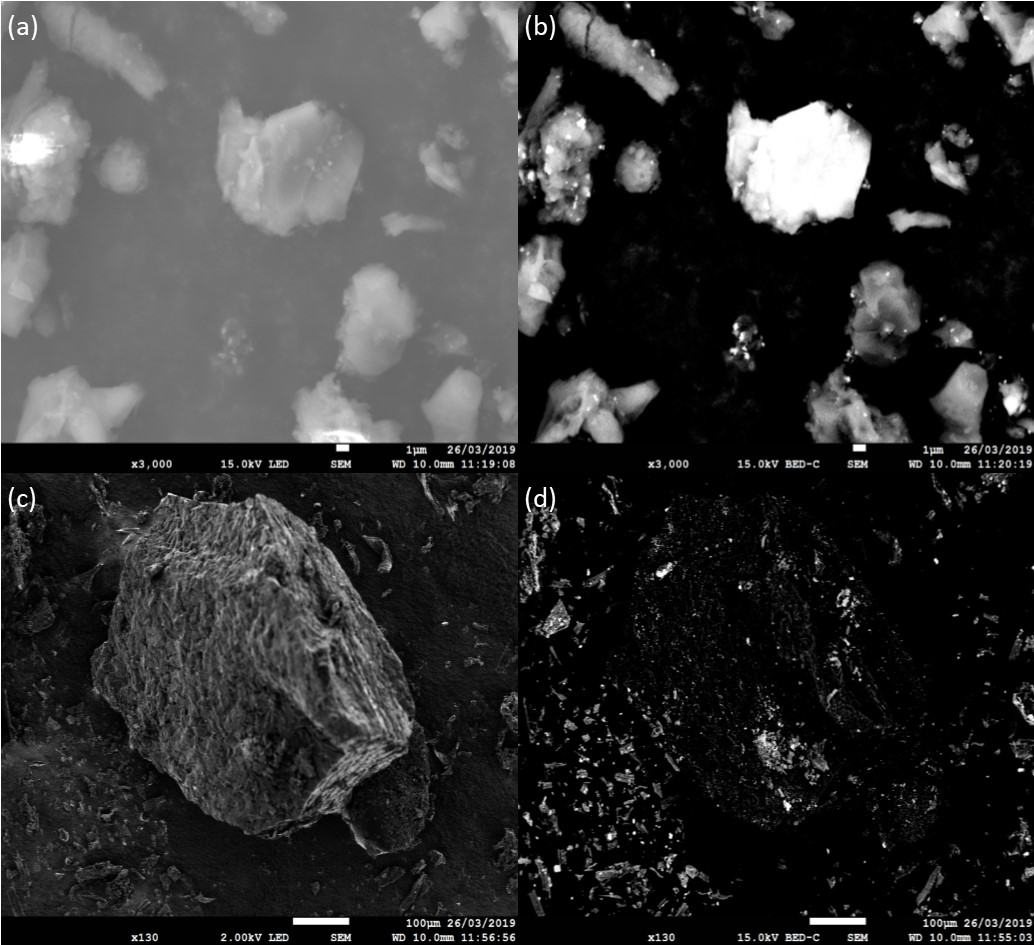
\includegraphics[width=\columnwidth, keepaspectratio]{4-cbs/figs/SEM_BSE.png}
    \caption{SE (a, c) and BSE (b, d) images of samples hD-hydrochar (a, b) and hD-0600$'$ (c, d).}
    \label{fig:SEM_BSE}
\end{figure}

\begin{figure}[b!]
    \centering
    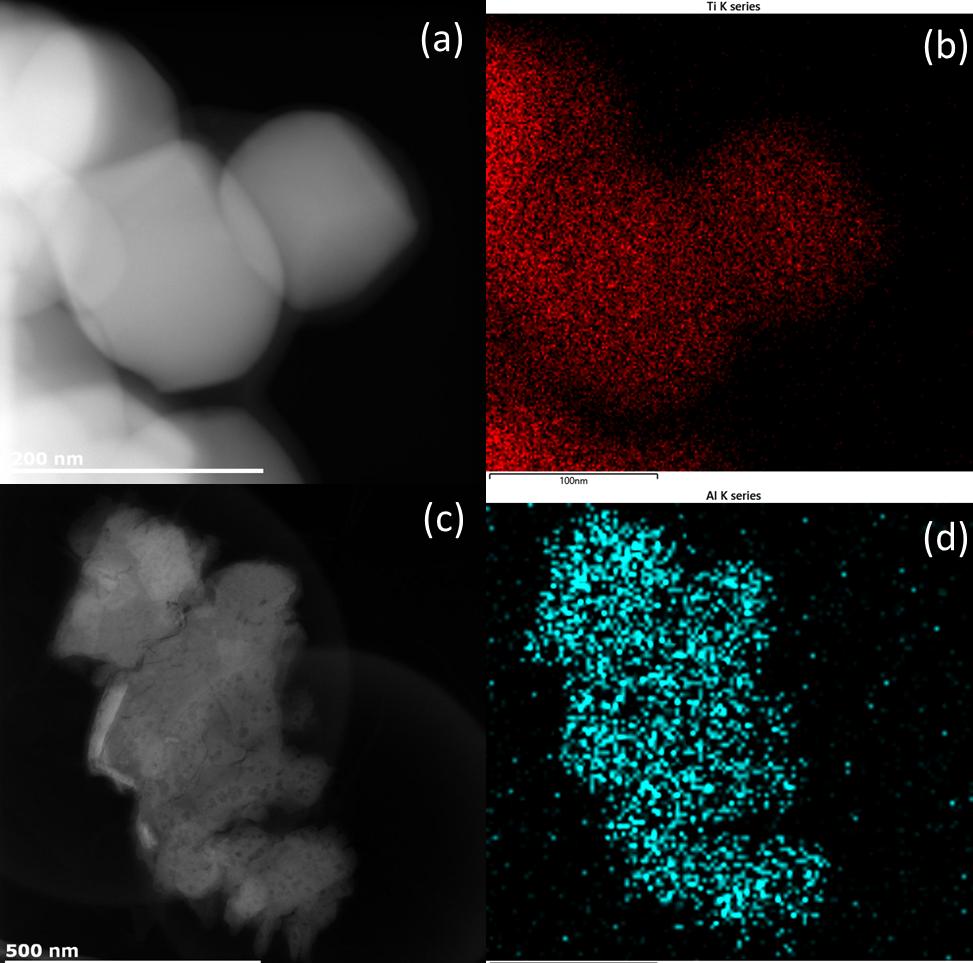
\includegraphics[width=\columnwidth, keepaspectratio]{4-cbs/figs/EDX_TEM.png}
    \caption{\acrshort{tem} (a, c) and \acrshort{edx}-\acrshort{tem} (b, d) images of hD-0700$'$ at sites 1 (a, b) and 3 (c, d). (b) and (d) show distribution of \ce{Ti} and \ce{Al} particles respectively.}
    \label{fig:EDX_TEM}
\end{figure}

For more detailed analysis of the distribution of elements in \glspl{turbostratic carbon}, EDX-TEM was used. Representative images derived using this technique are shown in figure \ref{fig:EDX_TEM}, and quantification at three different sites in table \ref{tb:cb_edx}. Most of the elements quantified by ICP-OES; \ce{Al}, \ce{Ca}, \ce{Cu}, \ce{K}, and \ce{Ti} are also identifiable by EDX-TEM, the \ce{Fe} and \ce{Na} are notably absent. In addition, \ce{Au} and \ce{Cr} are also present, though not in quantifiable amounts. The images in figure \ref{fig:EDX_TEM} show that heavy elements in the \glspl{turbostratic carbon} form clusters over the surface of the carbon structure. \ce{Ti} and \ce{Al} are the only metals whose concentrations were quantifiable at any site examined, with site 2 having \ce{Ti} as the majority component. \ce{Al} could only be quantified at site 3, wherein \ce{Ti} was notably absent in measurable quantities. Thus, it appears that at \ce{Ti} and \ce{Al} form discrete clusters within this \gls{turbostratic carbon}. On the other hand, the other metals identified by \acrshort{icp-oes} (see table \ref{tb:icp}) must be distributed more evenly meaning that they can not be as readily quantified in the small (roughly \qty{100}{\micro\metre\squared}) sites examined.

\begin{table}[t!]
    \caption{Concentrations of \ce{C}, \ce{O}, \ce{Al} and \ce{Ti} at three different sites in hD-4700 according to EDX-TEM }
    \label{tb:cb_edx}
    \begin{tabularx}{\textwidth}{llXlXlX}
    \toprule
        \textbf{Analyte} & \multicolumn{6}{c}{\textbf{Concentration / \unit{\wtpercent} (Atomic \unit{\percent})}} \\
        & \multicolumn{2}{l}{\textbf{Site 1}} & \multicolumn{2}{l}{\textbf{Site 2}} & \multicolumn{2}{l}{\textbf{Site 3}} \\
    \midrule
        \textbf{\ce{C}} & 80 & (90) & 33 & (36) & 73 & (82)\\
        \textbf{\ce{O}} & 8 & (7) & 4 & (5) & 14 & (12) \\
        \textbf{\ce{Al}} & - & (-) & - & (-) & 3 & (2) \\
        \textbf{\ce{Ti}} & 10 & (3) & 60 & (29) & - & (-) \\
    \bottomrule
    \end{tabularx}
\end{table}



\subsection{Porosity}

\begin{table}[hb!]
    \centering
    \caption{Porosity of \acrshort{ucb}-derived carbons from \ce{N2} isotherms. $A_{BET}$ determined using the Rouquerol method where applicable. Total pore volume, $V_t$ determined using the single point method. Numbers in brackets indicate micropore surface area and pore volume. Peak pore width, $w_{peak}$ (for samples hC-4\textit{TTT} and hD-4\textit{TTT}) taken as peak of the \acrshortpl{psd} in figure \ref{fig:cb_isopsd}.}
    \label{tb:cb_porosity}
    \begin{tabularx}{0.9\textwidth}{lllllll}
    \toprule
        \textbf{Sample} & \multicolumn{2}{l}{$\mathbf{A_{BET}}$ \textbf{/ \unit[detect-weight]{\metre\squared\per\gram}}}  & \multicolumn{2}{l}{$\mathbf{V_t}$ \textbf{/ \unit[detect-weight]{\cm\cubed\per\gram}}} & \multicolumn{2}{l}{$\mathbf{w_{peak}}$ \textbf{/ \unit{\angstrom}}} \\
    \midrule
        \textbf{hD-0600$'$} & 10 & (-) & - & (-) & \\
        \textbf{hD-0700$'$} & 170 & (150) & 0.07 & (0.06) \\
        \textbf{hD-0800$'$} & 226 & (198) & 0.09 & (0.08) \\
        & & & \\
        \textbf{hD-0600} & 120 & (104) & 0.05 & (0.04) & \\
        \textbf{hD-0700} & 122 &  (101) & 0.05 & (0.04) & \\
        \textbf{hD-0800} & 146 & (125) & 0.06 & (0.05) \\
        & & & \\
        \textbf{hC-4600} & 1428 & (1054) & 0.63 & (0.43) & 7  \\
        \textbf{hD-4600} & 1487 & (1036) & 0.64 & (0.41) & 7 \\
        & & & \\
        \textbf{hC-4700} & 1875 & (917) & 0.89 & (0.37) & 8 \\
        \textbf{hD-4700} & 1807 & (611) & 0.88 & (0.25) & 9  \\
        & & & \\
        \textbf{hC-4800} & 1958 & (626) & 1.00 & (0.26) & 8 \\
        \textbf{hD-4800} & 979 & (206) & 0.52 & (0.09) &  8 \\
    \bottomrule
    \end{tabularx}
\end{table}

As a result of the discovery of high quantities of non-combustible matter in turbostratic carbons which both were and were not washed, the effect of the washing step on porosity was examined. The results, i.e. porosity of samples hD-0\textit{TTT} and hD-0\textit{TTT}$'$ are shown in table \ref{tb:cb_porosity} alongside that for sets hC-4\textit{TTT} and hD-4\textit{TTT}. Isotherms and resultant PSDs for samples hC-4\textit{TTT} and hD-4\textit{TTT} are displayed in figure \ref{fig:cb_isopsd}.\footnote{Isotherms and PSDs for hD-0\textit{TTT} and hD-0\textit{TTT}$'$ can be found in the appendix, figure \ref{fig:0TTT_psdiso}, as well as full plots of isotherms and fits for all samples for which porosity is reported herein in figures \ref{fig:4TTT_psdisofull} and \ref{fig:0TTT_psdisofull}. Due to poor equilibration, the PSDs cannot be considered to be accurate. This issue is discussed in more depth in chapter \ref{ch:dual_isotherm} and \ref{pub:dual_iso}.}.  It is unclear whether washing in \ce{HCl} had any effect at all on porosity - indeed, for activation at 700 and \qty{800}{\degreeCelsius} there are significant reductions in $A_{BET}$ after washing. Perhaps this is simply a marker of physical agglomeration of particles during the washing process, and has little to do with internal porosity. Additionally, the porosity of these samples is not higher than would be expected for pyrolysed biomass; \gls{self-activation} of a pure cellulose acetate-derived \gls{hydrochar} yielded a carbon with $A_{BET}$  \qty{>500}{\metre\squared\per\gram},\footnote{Full porosimetric details of this sample are in appendix, figure \ref{fig:CA_psdiso} and table \ref{tb:CA_porosity}.} indeed \acrshort{ucb}-derived self-activated carbons have previously been shown to exhibit far higher surface areas.\citep{Soltani2013, Yazdi2012, Lee2014, Yu2018, Koochaki2019} As such there is no proof that the non-combustible contaminants can act as \glspl{porogen}. Of course this is not definitive as removal of contaminants proved impossible in these samples. The porosity that hD-0\textit{TTT} carbons \textit{do} possess is principally (over \qty{80}{\percent}, by surface area) in the \gls{micropore} region, though again this is to be expected for \glspl{biochar}/self-activated carbons.\citep{Weber2018Properties, Jagiello2019Enhanced, suliman2017role}

\begin{figure}[t]
    \centering
    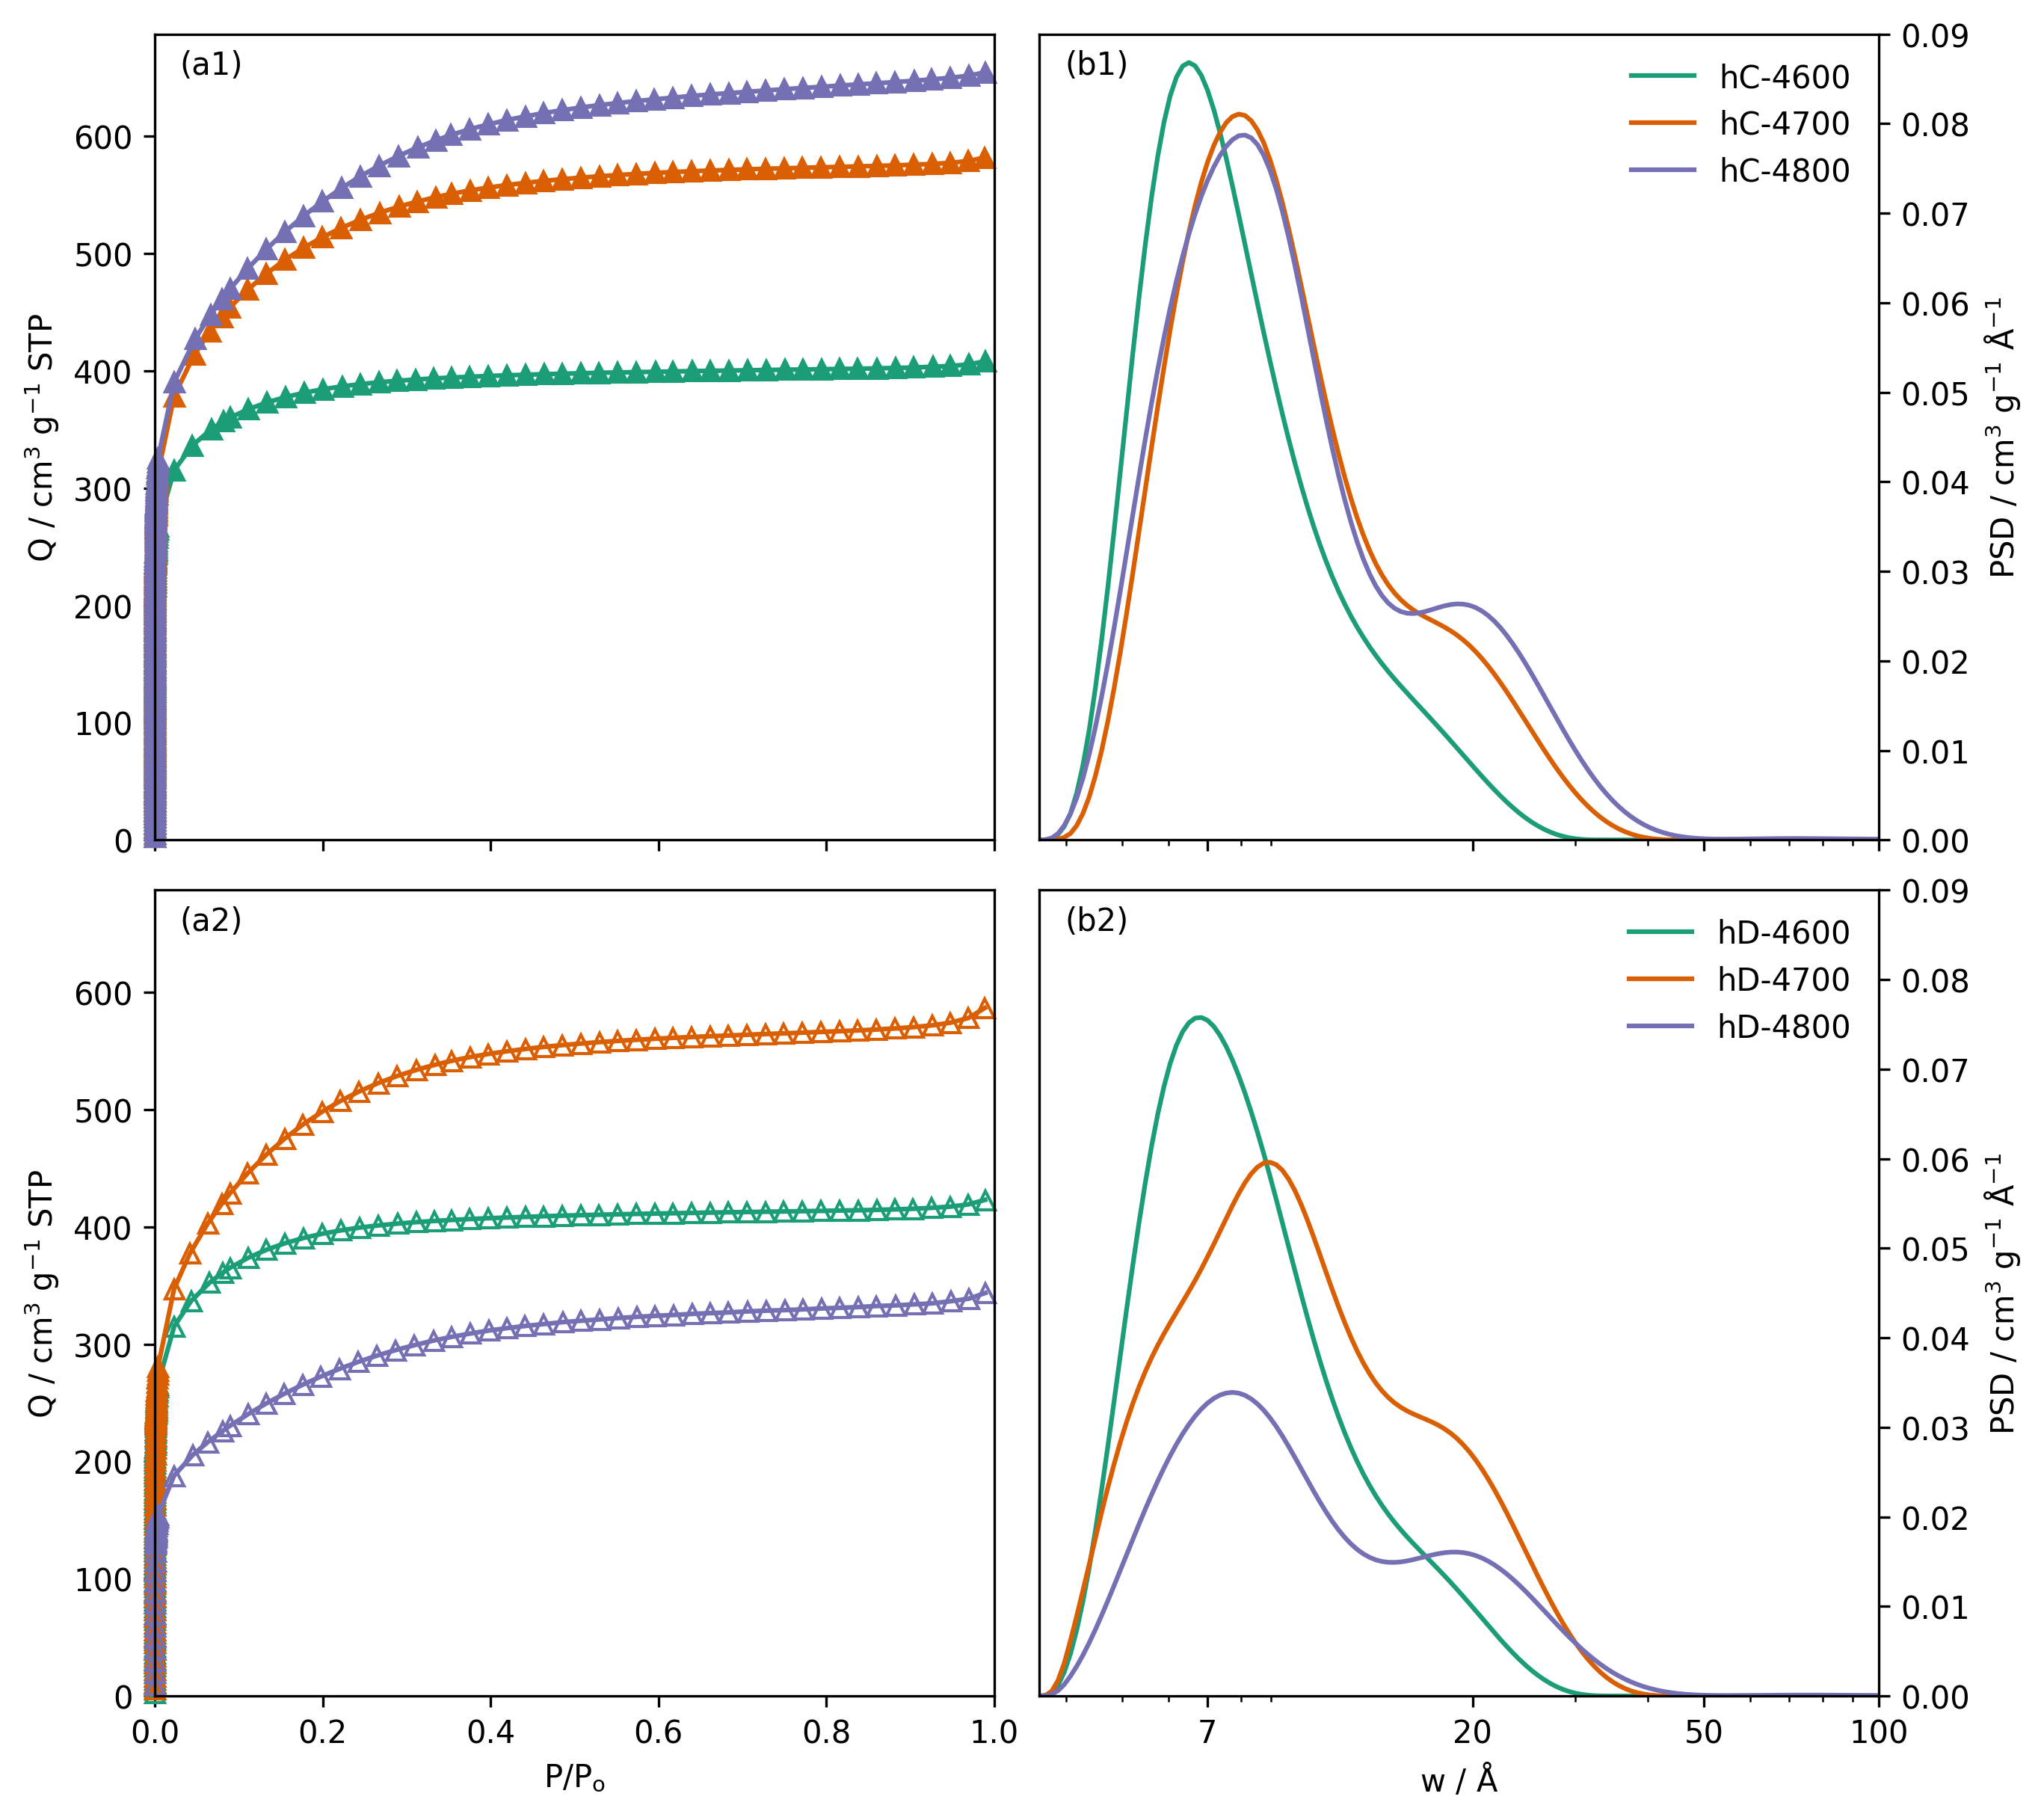
\includegraphics[width=\columnwidth, keepaspectratio]{4-cbs/figs/CB_n2_isotherms.png}
    \caption{Isotherms and resultant PSDs for samples hC-4\textit{TTT} and hD-4\textit{TTT}.}
    \label{fig:cb_isopsd}
\end{figure}

Carbons activated using \ce{KOH} have moderate surface areas, and a much lower relative microporosity than samples hD-0\textit{TTT}, ranging from \qty{71}{\percent} to as low as \qty{21}{\percent} when activated at \qtylist[list-units=single]{600;800}{\degreeCelsius} respectively. That is, these carbons are much more mesoporous, and mesoporosity increases with activation temperature. Indeed, the mesoporosity is reflected in the broad curvature of the \ce{N2} isotherms used to determine these textural characteristics as show in figure \ref{fig:cb_isopsd}(a1, a2). This is in contrast to the carbons reported in \ref{pub:CB}, where the author reported $A_{BET}$ of more than double that shown in this work, and all carbons were mostly microporous. This is likely a result of the relatively high (estimated) oxygen content, and thus low activation resistance (see \ref{pub:review}, \textbf{section 4.1.2.}) of the \glspl{hydrochar} formed in this work (see table \ref{tb:chn_ash}) as opposed to any limitations on porosity development resulting from the non-combustible contaminants. The lowest possible estimates of O-content for hC-hydrochar and hD-hydrochar are \qtylist[list-units=single]{37;35}{\wtpercent} respectively,\footnote{Minimum O-content taken as the difference between `other' and \gls{ash content} of the \glspl{hydrochar} (table \ref{tb:chn_ash}). The true value is likely much higher as the ash contains the oxides of non-combustible contaminants, thus weight reported is greater than in the carbon itself.} compared to \qty{25}{\wtpercent} for \acrshort{ucb}-derived \gls{hydrochar} in \ref{pub:CB}. 


Washing of the \gls{hydrochar} does not appear to have a consistent effect on porosity of derived KOH-activated carbons. That is,  $A_{BET}$ and pore volume are the essentially the same for both sets of carbons activated with \ce{KOH} at \qtylist[list-units=single]{600;700}{\degreeCelsius}, while porosity of hD-4800 is approximately half that of hC-4800. On the other hand, activation at \qtylist[list-final-separator={or }, list-units=single]{700;800}{\degreeCelsius} of unwashed \gls{hydrochar} results in much lower absolute microporosity relative to washed \gls{hydrochar}. This may be a result of combustion of volatile compounds dried into the unwashed \gls{hydrochar}, which produces oxidising gases such as \ce{CO} and \ce{CO2} leading to uncontrolled degradation of the carbon framework, and thus pore broadening.\citep{Sevilla2014Energy, Blankenship2022Modulating} This pore width broadening with increasing activation temperature is also evidenced by the PSDs of the carbons (see figure \ref{fig:cb_isopsd}(b1, b2)), with significantly more of the porosity above 20 \AA\space for samples activated at \qtylist[list-final-separator={or }, list-units=single]{700;800}{\degreeCelsius} relative to \qty{600}{\degreeCelsius}. The pores also become centered around higher values of $w$ (see table \ref{tb:cb_porosity}) with increasing activation temperature, though this trend is somewhat obscured for samples hD-4\textit{TTT} - but this may simply be an effect of reduction in overall porosity resulting from combustion of volatiles in the activation process. Pore size hierarchy does not appear to be significantly affected by the presence (or lack of) a \gls{hydrochar} washing step.

\subsection{\texorpdfstring{\ce{CO2} uptake}{CO2 uptake}}

While the ultra-high surface areas of carbons reported in \ref{pub:CB} made them excellent candidates for \ce{H2} storage, this is not the case for \acrshort{ucb}-derived KOH-activated carbons prepared in this work. The lower surface area and more hierarchical pore structure of these carbons (table \ref{tb:cb_porosity}) make them much better candidates for \ce{CO2} capture. As such, room temperature molar \ce{CO2} uptake was measured up to \qty{40}{\bar}, and results thereof are tabulated in table \ref{tb:cb_co2} and shown in full in figure \ref{fig:cb_co2}. 

\begin{table}[b!]
    \centering
    \caption{\ce{CO2} uptakes (measured at \qty{25}{\degreeCelsius}) at \qtylist[list-units=single]{1;20}{\bar} for samples hC-4\textit{TTT} and hD-4\textit{TTT}.}
    \label{tb:cb_co2}
    \begin{tabularx}{0.8\textwidth}{XXX}
    \toprule
        \textbf{Sample} & \multicolumn{2}{c}{\textbf{\ce{CO2} uptake / \unit[detect-weight]{\milli\mole\per\gram}}} \\
         & \textbf{1 \unit[detect-weight]{\bar}} & \textbf{20 \unit[detect-weight]{\bar}}\\
    \midrule
        \textbf{hC-4600} & 2.6 & 9.8 \\
        \textbf{hD-4600} & 1.5 & 6.1 \\
        \\
        \textbf{hC-4700} & 2.3 & 12.1 \\
        \textbf{hD-4700} & 2.3 & 14.1 \\
        \\
        \textbf{hC-4800} & 2.7 & 12.6 \\
        \textbf{hD-4800} & 1.5 & 9.7 \\
    \bottomrule
    \end{tabularx}
\end{table}

\begin{figure}[hb!]
    \centering
    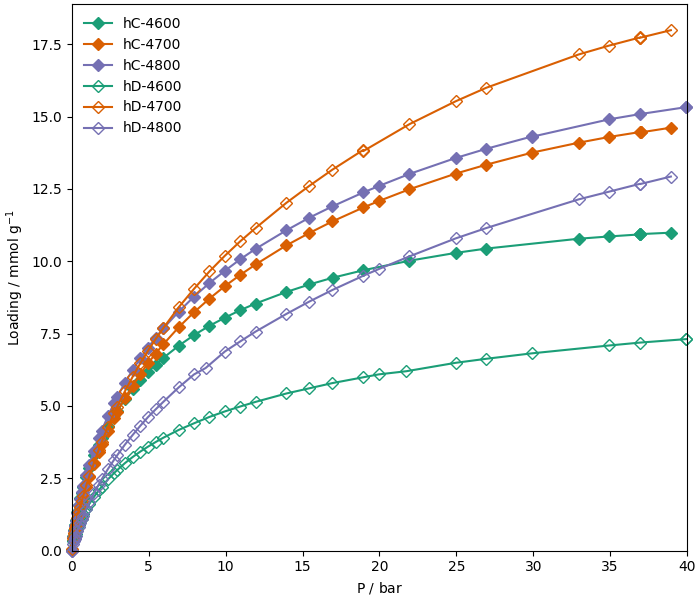
\includegraphics[width=\columnwidth, keepaspectratio]{4-cbs/figs/CB_CO2.png}
    \caption{\ce{CO2} uptake isotherms (298 K) for samples hC-4\textit{TTT} and hD-4\textit{TTT}.}
    \label{fig:cb_co2}
\end{figure}

At \qty{20}{\bar}, the highest surface area samples - hD-4700, hC-4700 and hC-4800 - perform the best as a result of maximisation of available adsorption sites for attractive London forces between \ce{CO2} and the material surface. The more mesoporous hD-4700 (see table \ref{tb:cb_porosity}) has a \qty{17}{\percent} greater \ce{CO2} uptake than the more microporous hC-4700 at \qty{20}{\bar}. This is likely because \glspl{mesopore} fill at higher pressure than \glspl{micropore}. Conversely, if we compare hC-4600 and hD-4600 the origin of the discrepancy in their \ce{CO2} uptake is unclear at both 1 and 20 bar, as their porosity is essentially identical. The only major distinction is compositional; hD-4600 has a far higher \gls{ash content} (see table \ref{tb:chn_ash}). Perhaps some contaminant prevents ingress of \ce{CO2} into hD-4600's pores. Optimum low pressure \ce{CO2} uptake is achieved by two samples with quite different porosity; hC-4600 and hC-4800. The high degree of microporosity ($A_{BET} = \qty{1023}{\metre\squared\per\gram}$, $V_t = \qty{0.64}{\cm\cubed\per\gram}$) in hC-4600 counteracts the greater overall porosity of hC-4800, whose pore volume is \qty{56}{\percent} greater than hC-4600. 

The \ce{CO2} uptakes of the two samples synthesised at \qty{600}{\degreeCelsius} approach a plateau at pressures in excess of \qty{10}{\bar}. This behaviour is likely a result of the fairly narrow \acrshortpl{psd} of these carbons. On the other hand, the slope of isotherms for the other four samples does not decrease to the same extent as they have a greater degree of hierarchy in their \acrshortpl{psd}. Thus the samples synthesised at \qtylist[list-units=single]{700;800}{\degreeCelsius} are more suitable for applications such as \acrshort{psa}.\citep{Sevilla2014Energy} The activation temperature-porosity-gas uptake capacity relationship is similar to that for carbons synthesised in \ref{pub:CA} and \ref{pub:CB}, in that optimum porosity for \ce{CO2} uptake is achieved at a lower than expected activation temperature of \qty{700}{\degreeCelsius}. In general in a series of \glspl{turbostratic carbon} derived through the activation of biomass, the optimum gas uptake is achieved for samples activated at \qty{\sim800}{\degreeCelsius}.\citep{Ariharan2018}

\section{Conclusion}

The KOH-mediated pyrolysis of whole \acrshortpl{ucb} does not yield carbons with ultrahigh porosity as shown in \ref{pub:CB}. This appears to be due to compositional differences, i.e. that the wrapping paper is not as readily activated as the \acrshort{ca} present in the filters themselves. As a result, KOH-activated materials do not show promise as \ce{H2} storage media, but instead their medium $A_{BET}$ (approaching \qty{2000}{\metre\squared\per\gram}) and hierarchical \acrshortpl{psd} make them useful for ambient temperature \ce{CO2} capture; \ce{CO2} uptakes of \qtylist[list-units=single]{2.7;14.1}{\milli\mole\per\gram} were achieved at \qtylist[list-units=single]{1;20}{\bar} respectively. 

Of further interest is the function of the two washing steps, i.e. after \gls{htc} and after pyrolysis. It appears that removal of non-combustible contaminants is inconsistent, although washing the \gls{hydrochar} \textit{does} remove volatile organic matter, which may slightly increase the concentration of \ce{C} in derived turbostratic carbons. On the other hand, washing of the carbons pyrolysed in the absence of KOH has inconsistent effects on porosity, and indeed on the concentration of non-combustible matter in the samples with \glspl{ash content} of up to \qty{20}{\wtpercent} even in washed carbons. In addition the porosity of these samples is lower than is found for carbon derived from the sequential \gls{htc} and pyrolysis of pure \acrshort{ca}, suggesting some interference of the stubborn metal contaminants with pore accessibility.

The difficulty in the removal of non-combustible contaminants led the author to investigate their nature. It was found through a combination of \acrshort{icp-oes}, \acrshort{xps}, and electron microscopy that \ce{Al}, \ce{Fe}, \ce{K}, \ce{Mg}, \ce{Na}, \ce{Ti}, and \ce{Ca} are present in whole \acrshortpl{ucb} and unwashed \gls{hydrochar}. In addition, nanoclusters of \ce{Au} and \ce{Cr} were also identified in an unwashed \gls{turbostratic carbon}. 

\bibliographystyle{rsc}
\bibliography{bibliography/bib}